\section{Detección óptima, filtro acoplado}

Replanteamos el problema del diseño del filtro de recepción $H_R$
(denotado aquí por $H$) buscando la mínima probabilidad de error
debida al ruido, ignorando por ahora la ISI. En vez de ``dejar
pasar'' la señal, permitimos que el pulso se distorsione en el
filtro; el objetivo es que en el momento de muestreo el pulso de
salida tenga amplitud máxima en relación al ruido.

Supongamos que a la entrada de $H$ llega un pulso $a_0 p(t)$,
contaminado con ruido blanco $\frac{\eta}{2}$. Aquí $a_0$ puede
ser unipolar ($\{0,A\}$) o polar ($\pm A$), y el pulso de energía
finita tiene forma conocida pero arbitraria.

A la salida del filtro de respuesta impulsiva $h(t)$  y respuesta
en frecuencia $\hat{H}(f)$, tendremos $a_0 p(t) \ast h(t) + n(t)$
donde $n(t)$ es un ruido de media $0$, varianza
$\sigma^2=\frac{\eta}{2}\displaystyle{\int_{-\infty}^{+\infty}
|\hat{H}(f)|^2\d f}$.



Muestreo en $t=\tau$. La señal muestreada es $a_0(p\ast h)
(\tau)$, que toma valores ($\{0,A'\}$) o ($\pm A'$), siendo
$A'=A(p\ast h)(\tau)$. La probabilidad de error de detección $P_e$
estará entonces determinada por la relación $\frac{A'}{\sigma}$,
expresamos su cuadrado a continuación:
%
\[\left(\frac{A'}{\sigma}\right)^2 = \frac{2 A^2 |(p\ast
h)(\tau)|^2}{\eta \int_{-\infty}^{+\infty} |\hat{H}(f)|^2\d f}.\]
Buscamos maximizar lo anterior (para minimizar $P_e$) pero esto no
es inmediato ya que el filtro $H$ aparece en el numerador y
denominador. Para llegar a una expresión más clara escribimos
numerador en términos de la transformada de Fourier $\hat{H}(f)$.

\begin{gather*}
    (p\ast h) \stackrel{\mathcal{F}}{\longrightarrow} \hat{P}(f) \hat{H}(f)\\
    \Rightarrow (p\ast h)(\tau) = \int_{-\infty}^{+\infty} \hat{P}(f)
\hat{H}(f) \e^{j2\pi f \tau}\d f.
\end{gather*}

\paragraph{Llegamos al siguiente problema de optimización:}

\begin{equation}
    \label{eq:op}
    \max_{\hat{H}(f)} \frac{\left|\displaystyle\int_{-\infty}^{+\infty}
\hat{P}(f) \hat{H}(f) \e^{j2\pi f \tau}\d
f\right|^2}{\displaystyle\int_{-\infty}^{+\infty} |\hat{H}(f)|^2\d
f}. \tag{*}
\end{equation}

Como la optimización tiene $\infty$ grados de libertad
(optimización en todos los filtros) no es de solución obvia. Sin
embargo se la puede resolver recurriendo a la desigualdad de
Cauchy-Schwarz (válida para toda función de cuadrado integrable):
%con igualdad $\Leftrightarrow \hat{V} = K \hat{W}$):
\[\left|\left\langle\hat{V}(f),\hat{W}(f)\right\rangle\right|^2 \leq ||\hat{V}||^2
||\hat{W}||^2, \quad \text{ con igualdad }\Leftrightarrow \hat{V}
= K \hat{W}.\] O sea:
\[\left|\int \hat{V}(f) \overline{\hat{W}(f)}\d f\right|^2\leq \int_{-\infty}^{+\infty}
|\hat{V}(f)|^2\d f \int_{-\infty}^{+\infty} |\hat{W}(f)|^2\d f.\]
Tomemos aquí $\hat{V}(f) = \hat{H}(f)$, $\overline{\hat{W}(f)} =
\hat{P}(f)\e^{j2\pi f \tau}$. Usando la desigualdad tenemos
%
\[
\frac{\left|\displaystyle\int_{-\infty}^{+\infty} \hat{P}(f)
\hat{H}(f) \e^{j2\pi f \tau}\d
f\right|^2}{\displaystyle\int_{-\infty}^{+\infty} |\hat{H}(f)|^2\d
f} = \frac{\left|\left\langle
\hat{V},\hat{W}\right\rangle\right|^2}{||\hat{V}||^2}\leq
||\hat{W}||^2 = \int_{-\infty}^{+\infty} |\hat{P}(f)|^2\d f =
||p||^2.\]
O sea que el máximo en \eqref{eq:op} es acotado, y la
igualdad se alcanza sólo si
\[\hat{H}(f) = K\overline{\hat{P}(f)}\e^{-j2\pi f \tau} \Rightarrow h(t)=K
p\left(-(t-\tau)\right)\Rightarrow \col{h(t) = K p(\tau-t)}.\]

\begin{figure}[htb]
    \centering\begin{minipage}{\textwidth}
    \bpgf{Imagenes/filAc/filAc-1}
    \begin{tikzpicture}
        \draw[->] (-0.5,0) -- (4,0) node [anchor=north] {$t$};
        \draw[->] (0,-0.5) -- (0,1.5);
        \draw (0,0) -- (2,1) -- (3,0);
        \path (5,1) node {$\Rightarrow$};
        \begin{scope}[shift={(6,0)}]
                \draw[->] (-0.5,0) -- (4,0) node [anchor=north]
{$t$};
                \draw[->] (0,-0.5) -- (0,1.5) node [anchor=west]
{$h_{opt} = K p(\tau - t)$};
                \draw (0.5,0) -- (1.5,1) -- (3.5,0) node
[anchor=north] {$\tau$};
        \end{scope}
    \end{tikzpicture}
    \endpgfgraphicnamed\end{minipage}
\end{figure}
\FloatBarrier

Concluimos que la respuesta impulsiva del filtro \'optimo tiene la
forma del pulso incidente, invertido en el tiempo: se dice que el
filtro \'optimo est\'a {\bf acoplado (o apareado)}  al pulso.

Para interpretar el resultado en el dominio del tiempo, conviene
escribir el pulso de salida $p_R =h\ast p$ para el filtro
\'optimo:
\begin{align*}
            p_R(t) = (h\ast p) (t)  & = \int_{-\infty}^{+\infty}
h(t-\sigma) p (\sigma)\d \sigma\\
                        & =
%\frac{1}{||p||^2}
K \int_{-\infty}^{+\infty} p(\tau - t + \sigma) p (\sigma)\d
\sigma \\ & = K r_p(t - \tau).
        \end{align*}
Aquí $r_p(\cdot)$ es la autocorrelaci\'on del pulso como señal de
cuadrado integrable. Como la autocorrelación es máxima en cero, el
pulso de salida toma su amplitud máxima en el instante de muestreo
$t=\tau$. En otras palabras: el detector basado en este filtro y
muestreo en $t=\tau$ est\'a {\em correlacionando} la señal de
entrada $a_0 p(t) + n(t)$ con la forma de onda conocida del pulso.


\begin{remarksSN}
    $\phantom{1}$
    \begin{enumerate}
        \item La constante $K$ es arbitraria, escalar el filtro no
        cambia el cociente de \eqref{eq:op}. Una elección cómoda es
$K=\dfrac{1}{||p||^2}=\dfrac{1}{r_p(0)}$: de ese modo el pulso de
salida $p_R(t)$ tiene valor m\'aximo igual a 1, alcanzado en
$t=\tau$. En ese caso la amplitud $A'$ de muestreo coincide con la
amplitud $A$ de los s\'imbolos de entrada.
        \item $\tau$ sería idealmente arbitrario, excepto que en la
práctica queremos $h(t)$ causal. Entonces tomo $\tau$ igual a la
duración del pulso $p(t)$ (si $p(t)=\sinc$ hay que truncarlo).
    \end{enumerate}
\end{remarksSN}

El máximo de nuestro problema de optimización es $\|p\|^2$. Por
tanto tenemos
\[
\left(\dfrac{A'}{\sigma}\right)^2_{\text{max}} = 2
\frac{A^2}{\eta} ||p||^2.\]
% Los libros tienen una generalización para ruido coloreado, $S_n(f)$.

A partir de esta fórmula podemos escribir la probabilidad de error
en términos de la energía media del pulso recibido,
$\overline{E}_p = E[a_k^2] ||p||^2$, en los distintos casos.

\begin{description}
    \item[Polar binario]
    \[\overline{E}_p = A^2 ||p||^2 \Rightarrow
\left(\frac{A'}{\sigma}\right)_\text{max} =
\sqrt{\frac{2\overline{E}_p}{\eta}} \Rightarrow P_e^\text{opt} =
Q\left(\sqrt{2\frac{\overline{E}_p}{\eta}}\right).\]
    \item[Unipolar binario]
    \[\overline{E}_p = \frac{A^2}{2}||p||^2 \Rightarrow
\left(\frac{A'}{\sigma}\right)_\text{max} = 2
\sqrt{\frac{\overline{E}_p}{\eta}} \Rightarrow P_e^\text{opt} =
Q\left(\sqrt{\frac{\overline{E}_p}{\eta}}\right).\]
 \end{description}

Estas fórmulas son iguales a las que obtuvimos para la detección
con pulsos de Nyquist, filtro pasabajos ideal. Esto no es
casualidad: para $p(t) = \sinc(\pi f_s t)$, el filtro acoplado es
un pasabajos ideal. O sea que en ese caso ya hicimos (sin saberlo)
lo óptimo. Pero las fórmulas valen para cualquier forma de pulso
con su detector apareado.

\subsection*{Caso M-ario polar} Ya se vio anteriormente que aquí la
probabilidad de error de símbolo es $P_e=2\frac{M-1}{M}
Q\left(\frac{A}{\sigma}\right)$. O sea que también aquí debemos
maximizar $\frac{A}{\sigma}$ y por tanto obtenemos el mismo filtro
acoplado. Escribimos la expresión en términos de $\overline{E}_p$
para este caso:
\begin{gather*}
 E[a_k]^2 = \frac{A^2 (M^2-1)}{3} \Rightarrow \overline{E}_p = A^2 \frac{(M^2-1)}{3}||p||^2
\Rightarrow \left(\frac{A'}{\sigma}\right)^2_{max} = \frac{6 \bar{E}_p}{\eta (M^2-1)}\\
\Rightarrow {\col{P_e^{opt} = 2\frac{M-1}{M}
Q\left(\sqrt{\frac{6\bar{E}_p}{\eta(M^2-1)}}\right)}}
\end{gather*}

\subsection*{Detector acoplado para pulsos rectangulares}

Tomemos por ejemplo los pulsos NRZ, $p(t) = p_{[0,T_s]}(t)$. El
filtro acoplado tendrá la respuesta impulsiva (tomando
$\tau=T_s$):
\[
\Rightarrow h(t) = \dfrac{1}{||p||^2} p(T_s-t) =
\dfrac{1}{T_s}p(t).
\]
\begin{minipage}{0.6\textwidth}
 A la salida del filtro se obtiene el pulso triangular
 \[p_R(t)=h(t)\ast p(t). \]
\end{minipage}
\begin{minipage}{0.4\textwidth}
 \begin{center}
  \bpgf{Imagenes/filAc/filAc-2}
    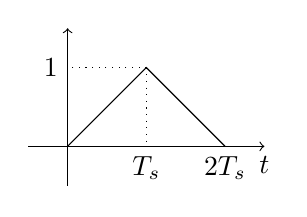
\begin{tikzpicture}
      \draw [->] (-0.5,0) -- (2.5,0) node [anchor=north] {$t$};
      \draw [->] (0,-0.5) -- (0,1.5);
      \draw (0,0) -- (1,1) -- (2,0) node [anchor=north] {$2T_s$};
      \draw [dotted] (1,1) -- (0,1) node [anchor=east] {$1$};
      \draw [dotted] (1,1) -- (1,0) node [anchor=north] {$T_s$};
    \end{tikzpicture}
  \endpgfgraphicnamed
 \end{center}
\end{minipage}

El filtro de recepción distorsionó fuertemente el pulso, pero esto
se  hizo de modo de maximizar $\frac{A}{\sigma}$ en el instante de
$t=T_s$ de muestreo.


\subsection*{¿Qué paso con la ISI?}

Al estudiar un solo pulso aislado, no contemplamos este tema.
Veamos:
\begin{itemize}
 \item En el caso pulsos de Nyquist ideales el detector acoplado es un pasabajos ideal, entonces los pulsos pasan intactos,
 sin ISI.
 \item En el caso de pulsos rectangluares NRZ. Vemos que $p_R(k T_s) = 0$ excepto en un valor ($k=1$). Entonces tampoco hay
 ISI.  Simplemente hay un retardo de $\tau = T_s$ al detectar.
 \item  De hecho, cualquier pulso de duración $\leq T_s$ (por ej., RZ) genera una $p_R(t)$ de duración $\leq
 2T_s$, que debidamente muestreado no genera  ISI.
\end{itemize}


\subsection*{Para pulsos de Nyquist con exceso de ancho de banda
$\alpha$}

El detector acoplado tiene respuesta en frecuencia
\begin{gather*}
 \hat{H}(f) = K \overline{\hat{P}(f)} \e^{-j2\pi f\tau}\\
 \Rightarrow \hat{P}_R = \hat{H}\hat{P} = K |\hat{P}(f)|^2 \e^{-j2\pi f \tau}
\end{gather*}
El último término es un retardo, afecta sólo el instante de
muestreo. A efectos de estudiar la ISI podemos tomar $P_R(f) =
K|\hat{P}(f)|^2$.
\begin{figure}[htb]
 \begin{center}\begin{minipage}{\textwidth}
  \bpgf{Imagenes/filAc/filAc-3}
  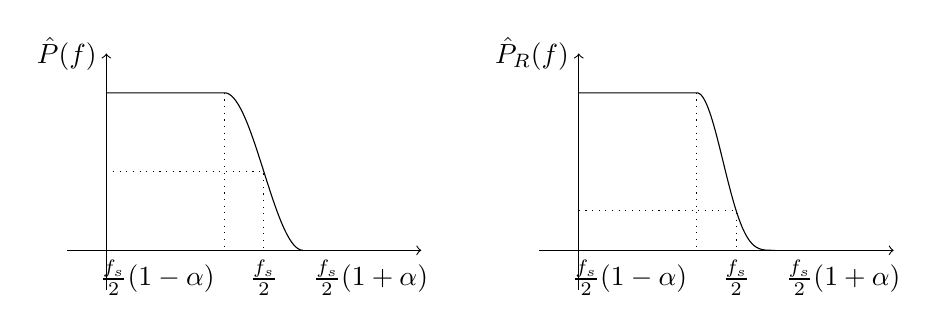
\begin{tikzpicture}
    \draw [->] (-0.5,0) -- (4,0);
    \draw [->] (0,-0.5) -- (0,2.5) node [anchor=east] {$\hat{P}(f)$};
    \draw  (0,2) -- (1.5,2) -- plot  [domain=1.5:2.5,samples=200] (\x,{cos(pi*(\x-1.5) r)+1});
    \draw [dotted] (1.5,2) -- (1.5,0) node [below left] {$\frac{f_s}{2}(1-\alpha)$};
    \draw [dotted] (0,1) -- (2,1) -- (2,0) node [below] {$\frac{f_s}{2}$};
    \path (2.5,0) node [below right] {$\frac{f_s}{2}(1+\alpha)$};
    \begin{scope}[shift={(6,0)}]
    \draw [->] (-0.5,0) -- (4,0);
    \draw [->] (0,-0.5) -- (0,2.5) node [anchor=east] {$\hat{P}_R(f)$};
    \draw  (0,2) -- (1.5,2) -- plot  [domain=1.5:2.5,samples=200] (\x,{(cos(pi*(\x-1.5) r)+1)^2/2});
    \draw [dotted] (1.5,2) -- (1.5,0) node [below left] {$\frac{f_s}{2}(1-\alpha)$};
    \draw [dotted] (0,0.5) -- (2,0.5) -- (2,0) node [below] {$\frac{f_s}{2}$};
    \path (2.5,0) node [below right] {$\frac{f_s}{2}(1+\alpha)$};
    \end{scope}
   \end{tikzpicture}
   \endpgfgraphicnamed\end{minipage}
 \end{center}

\end{figure}

$|\hat{P}(f)|^2$ no tiene simetría, entonces no cumple la condición de ISI nula.

O sea: poner el filtro óptimo desde el punto de vista del ruido,
me complica la ISI.

\newpage    %%% Solo para compilacion global.

Alternativas:
\begin{enumerate}
 \item En vez del $H_{opt}$, poner un pasabajos $(1+\alpha)\frac{f_s}{2}$, como ya se estudió. La $P_e$ da un poco peor,
 pero no introduzco ISI que sería más grave.
 \item Sabiendo que va a haber un filtro apareado, diseño $\hat{P}(f)$ para que $|\hat{P}(f)|^2$ no tenga ISI.
 Se usa a veces el pulso de {\bf raíz de coseno alzado.}
\end{enumerate}

%%%\newpage %% Va para compilar solo la parte digital
%% No va para el compilado global


\subsection*{Resumen: comunicación digital banda base}
\begin{figure}[htb]
    \centering
    \resizebox{\textwidth}{!}{%
    \bpgf{Imagenes/digBB/digBB-1}
    \begin{blockdiagram}
        \matrix[row sep=5mm, column sep=10mm]{
            & & \node[etiqueta] (ruido) {\large ruido blanco, $\frac{\eta}{2}$}; & & & & & \node[punto] (p1) {}; & \node [punto] (p2) {};\\
            \node[etiqueta] (inicio) {\large  $\sum_k a_k p_T(t-kT_s)$}; %& \node[block] (pulso) {$P_T(t)$};
             & \node[block] (canal) {\large CANAL} node[above=3mm] {
                    \begin{minipage}{2.2cm}
                       \large  (ancho de banda $B$)
                    \end{minipage}};
            & \node[operator] (sum) {$+$}; & \node [block] (filtro) {\large $\hat{H}_R(f)$} node [below=5mm] {
            \begin{minipage}{2.5cm}
                FILTRO DE\\RECEPCI�N
                \end{minipage}};
            & \node[punto] (p3) {} node [anchor=south] {\large $x_R(t)+n(t)$}; & \node [punto] (p4) {}; & & & \node[punto] (p5) {}; & \node [draw, isosceles triangle,thick] (comp) {
            \begin{minipage}{5mm}
                $+$\\$-$
            \end{minipage}};
            & \node[etiqueta] (salida) {\large $\{\hat{a}_k\}$};\\
            & & & & & & \node[block] (sinc) {\large SINCR}; & & \node [etiqueta] (v0) {$A_0$};\\
        };
        \draw [-stealth] (inicio) -- (canal);
        \draw [-stealth] (canal) -- (sum);
        \draw [-stealth] (ruido) -- (sum);
        \draw [-stealth] (sum) -- (filtro);
        \draw (filtro) -- (p3) -- (p4) -- (p2);
        \draw [-stealth] (p3) |- (sinc);
        \draw [-stealth] (sinc) -| (p1);
        \draw [-stealth] (p5) |- (comp.150);
        \draw [-stealth] (v0) |- (comp.south west);
        \draw [-stealth] (comp) -- (salida);
    \end{blockdiagram}
\endpgfgraphicnamed

    }
\end{figure}
\FloatBarrier

\begin{itemize}
 \item Transmito sucesión de pulsos $\sum a_k p_T(t-kT_s)$ (PAM)
 \item El canal introduce 2 distorsiones
\begin{enumerate}
  \renewcommand{\theenumi}{\roman{enumi}}
  \item \label{itemRes:1}Forma del pulso, por filtrado. Puede causar ISI.

  \item \label{itemRes:2}Ruido blanco.
\end{enumerate}
\end{itemize}

Si nos concentramos en (\ref{itemRes:1}), elegimos un pulso de
Nyquist y/o colocamos un \emph{ecualizador} en $\hat{H}_R(f)$.

Si nos concentramos en (\ref{itemRes:2}), ponemos en
$\hat{H}_R(f)$ el \emph{detector acoplado}.

Hay dos casos extremos en que las dos funciones se realizan
simultaneamente:

\begin{itemize}
 \item $p(t) = \sinc(\pi f_s t)$ (Nyquist ideal), $\hat{H}_R(f)$ pasabajos ideal. Se aplica a la situación:
    \begin{itemize}
     \item canal con $B$ muy restrictiva.
     \item puedo implementar la complejidad de pulsos/filtro.
    \end{itemize}
 \item $p(t)$ rectángular NRZ o RZ. Detector acoplado: $h_R(t) = \frac{1}{T_s}p(t)$. Se aplica a la situación:
\begin{itemize}
 \item $B$ muy grande (respecto a $f_s$).
  \item Implementación más simple. Sobre todo, el amplificador de transmisión puede ser no lineal.
\end{itemize}
\end{itemize}

En otros casos, puede existir conflicto entre los objetivos de
combatir las distorsiones (\ref{itemRes:1}) y (\ref{itemRes:2}).
Por ejemplo se vio que esto ocurría al usar pulsos de Nyquist con
exceso de ancho de banda. Aquí o se realiza un diseño conjunto de
$p_T$, $\hat{H}_R$, o sino se acepta una detección subóptima
respecto al ruido.
